\section{表象理论}

\begin{quotation}
``一个人永远不应该在知道一句化的结尾以前就开始说这句话。''\qquad 狄拉克
\end{quotation}

\begin{figure}[h]
\begin{center}
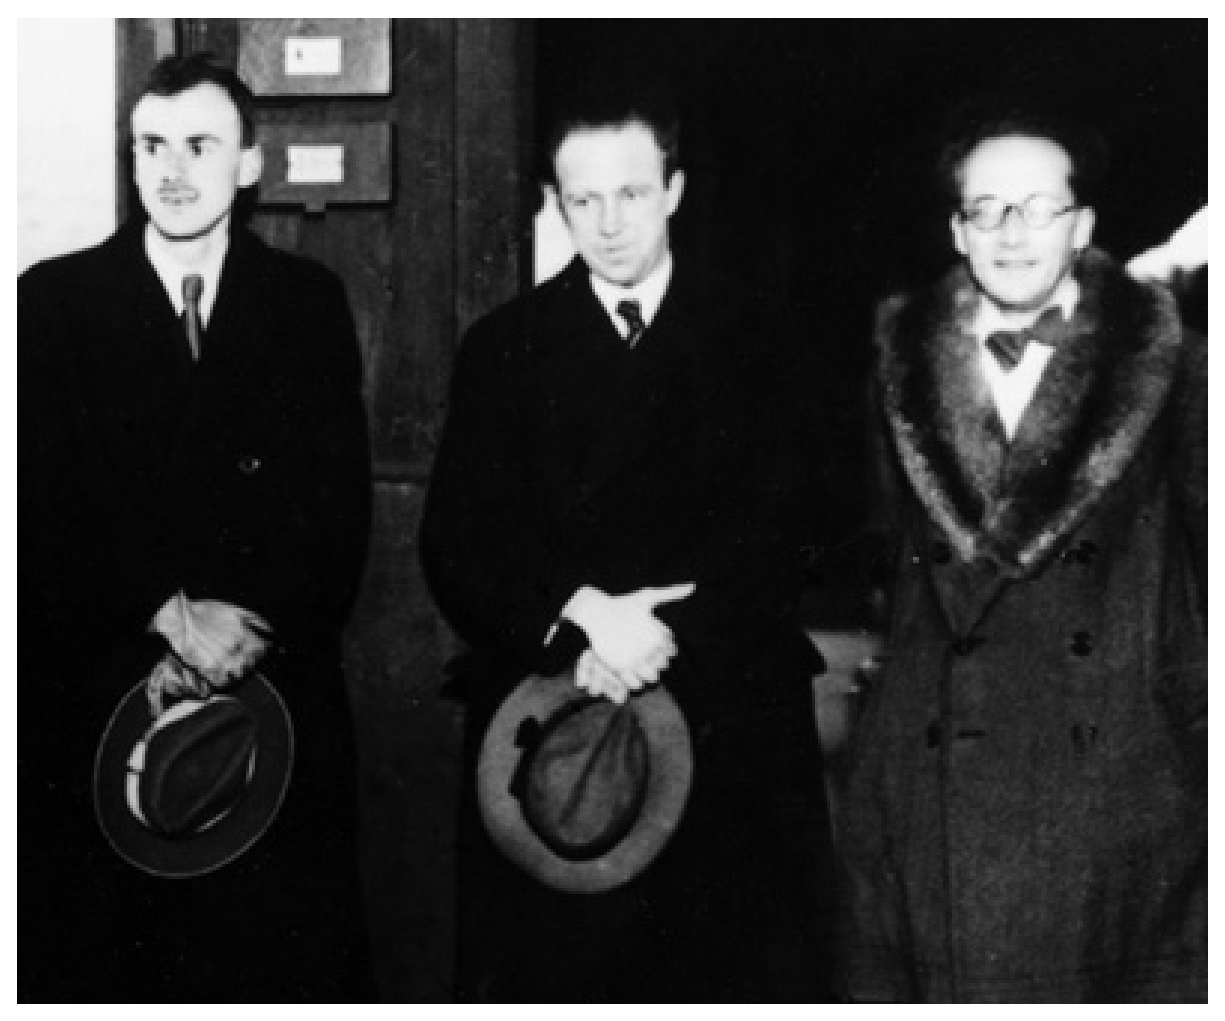
\includegraphics[clip,width=8cm]{Representations/1933nobel.ps}
\caption{量子力学的三个创立者:狄拉克、海森堡与薛定谔}
\end{center}
\end{figure}


\subsection{表象理论}


按照量子力学的理论, 微观粒子的运动状态用波函数$\psi$表示,
波函数$\psi$可以看作是Hilbert Space中的一个矢量,
波函数$\psi$随时间的演化满足薛定谔方程:$\widehat H\psi  = i\hbar
\frac{\partial }{{\partial t}}\psi $;

力学量用算符表示, 算符可以把Hilbert
Space中的一个矢量映射到另外一个矢量:

\begin{center}
$\varphi  = \widehat A\psi $, $\varphi ,\psi  \in {\rm{H}}$
\end{center}

$\widehat A\psi  = \lambda \psi $, $\lambda  \in {\rm{C}}$是算符$\hat A$的本征方程,本征值$\lambda$ 既可以是分立值,也可以是连续值,记作:$\lambda _n$;对应波函数的解记作:$\psi _n$,叫本征函数或本征矢。

由本征方程$\widehat A\psi  = \lambda \psi $,
可解出一组正交归一完备本征矢$\left\{ {\psi _n } \right\}$,满足:

$\left( {\psi _m ,\psi _n } \right) = \delta _{mn} $,或:$\left( {\psi _q ,\psi _{q'} } \right) = \delta \left( {q - q'} \right)$,(连续本征值)

以$\left\{ {\psi _n } \right\}$为基矢可以张开一个Hilbert Space,
由$\left\{ {\psi _n } \right\}$的完备性知, 任何波函数都可用$\left\{
{\psi _n } \right\}$的线性迭加表示:$\psi  = \sum\limits_n {a_n \psi
_n } $,$a_n  = \left( {\psi _n ,\psi } \right)$。$\left| {a_n }
\right|^2 $正是$\psi$所描写态中测量力学量$A$所得结果$\lambda
_n$的几率,所以迭加系数:$\left\{ {a_n }
\right\}$就是态矢$\psi$在$A$表象中的表示。

\index{Representation: 表象}

\subsubsection{态的矩阵表示}

我们可把任何态矢$\psi$表示为一个列矩阵的形式:

\index{Matrix representation: 矩阵表示}

\begin{equation}\label{19-1}
\psi  = \left( {\begin{array}{*{20}c}
   {a_1 }  \\
   {a_2 }  \\
   {...}  \\
\end{array}} \right)
\end{equation}

$\psi$的共轭矩阵可表示为一个行矩阵:

\begin{equation}\label{19-2}
\psi ^ +   = \left( {a_1^* ,a_2^* ,a_3^* ,...} \right)
\end{equation}

波函数的归一性:$\left( {\psi ,\psi } \right) = 1$,可表示为:

\begin{equation}\label{19-3}
\psi ^ +  \psi  = \sum\limits_n {\left| {a_n } \right|^2 }  = 1
\end{equation}


\subsubsection{算符的矩阵表示}

同样, 算符也可以表示为矩阵的形式;在$A$表象中, 任意算符$\hat
F$:$\varphi  = \widehat F\psi $,$\varphi ,\psi  \in {\cal
H}$;$A$表象:$\widehat A\psi _n  = \lambda _n \psi _n $,
可用正交归一完备本征矢$\left\{ {\psi _n } \right\}$展开:

$\psi  = \sum\limits_n {a_n \psi _n } $, $\varphi  = \sum\limits_m {b_m \psi _m } $

由$\sum\limits_m {b_m \psi _m }  = \widehat F\sum\limits_n {a_n \psi _n } $可求出$b_m$的表达: 

\begin{equation}\label{19-4}
b_m = \left( {\psi _m ,\widehat F\sum\limits_n {a_n \psi _n } } \right) = \sum\limits_n {\left( {\psi _m ,\widehat F a_n \psi _n } \right)}   = \sum\limits_n {F_{mn} a_n }
\end{equation}

这里:矩阵元$F_{mn}  = \left( {\psi _m ,\widehat F\psi _n } \right)$是算符$\hat F$在$A$表象中的表示。

可以证明算符$\hat A$在$A$表象中的表示是对角矩阵:

$A_{mn} = \left( {\psi _m ,\widehat A\psi _n } \right) = \left(
{\psi _m ,\lambda _n \psi _n } \right) = \lambda _n \delta _{mn} $




\subsubsection{矩阵的种类}

\begin{itemize}
    \item 对角矩阵:$A_{mn}  = \lambda _m \delta _{mn} $

\index{Diagonal matrix: 对角矩阵}

    \item 单位矩阵:$I_{mn}  = \delta _{mn} $, $IA = AI = A$

    \item 矩阵的复共轭:$\left( {A_{mn} } \right)^*  = A_{mn}^* $

\index{Complex adjoint: 复共轭}

    \item 矩阵的转置:$\widetilde{A_{mn} } = A_{nm} $

\index{Transpose: 转置}

    \item 矩阵的厄密共轭:$A_{mn}^ +   = A_{nm}^* $

\index{Hermitian adjoint: 厄米共轭}

    \item 厄密矩阵:$A_{mn}^ +   = A_{mn} $

    \item 幺正矩阵:$A^ +  A = I,A^ +   = A^{ - 1} $

\index{Unitary matrix: 幺正矩阵}

    \item 矩阵的迹(Trace):${\rm{Tr}}A = \sum\limits_n {A_{nn} } $

\index{Trace: 迹}

\begin{equation}\label{19-5}
Tr (AB) = \sum\limits_n {\left( {AB} \right)_{nn} }  = \sum\limits_{n,k} {A_{nk} B_{kn} }  = \sum\limits_{n,k} {B_{kn} A_{nk} }  = Tr(BA)
\end{equation}

   \end{itemize}

\subsubsection{本征方程的矩阵表示}

$\widehat F\psi  = \lambda \psi $, 在 表象中的表示:$\left( {\widehat F - \lambda \widehat I} \right)\psi  = 0$,即:

\begin{equation}\label{19-6}
\sum\limits_n {\left( {F - \lambda I} \right)_{mn} a_n }  = \sum\limits_n {\left( {F_{mn}  - \lambda \delta _{mn} } \right)a_n }  = 0
\end{equation}

有非零解的条件是系数行列式为零:$\det \left| {F_{mn}  - \lambda \delta _{mn} } \right| = 0$

\subsubsection{薛定谔方程}

$i\hbar \frac{\partial }{{\partial t}}\psi  = \widehat H\psi $, 在$A$表象中:

$i\hbar \frac{\partial }{{\partial t}}\sum\limits_m {a_m \psi _m }  = \widehat H\sum\limits_n {a_n \psi _n } $

$a_m$满足:

$i\hbar \frac{d}{{dt}}a_m  = \left( {\psi _m ,\widehat H\sum\limits_n {a_n \psi _n } } \right) = \sum\limits_n {\left( {\psi _m ,\widehat H\psi _n } \right)a_n }  = \sum\limits_n {H_{mn} a_n } $

\subsubsection{平均值公式}


$\overline F  = \left( {\psi ,\widehat F\psi } \right)$,在$A$表象中:

\begin{equation}\label{19-7}
\overline F  = \left( {\sum\limits_m {a_m \psi _m } ,\widehat F\sum\limits_n {a_n \psi _n } } \right) = \sum\limits_{mn} {a_m^* \left( {\psi _m ,\widehat F\psi _n } \right)a_n }  = \sum\limits_{mn} {a_m^* F_{mn} a_n }
\end{equation}

即:$\overline F  = \psi ^ +  F\psi $

\subsubsection*{练习1:坐标表象和动量表象}

\index{Coordinate representation: 坐标表象}

\index{Momentum representation: 动量表象}

考虑1维情形。坐标表象中:$\psi  = \psi \left( {x,t} \right)$,$\widehat x = x$,$\widehat p_x  = \frac{\hbar }{i}\frac{\partial }{{\partial x}}$

算符$\hat x$在$x$表象下的本征方程:$x\delta \left( {x - x'} \right) = x'\delta \left( {x - x'} \right)$

算符$\hat p$在$x$表象下的本征方程:

$\widehat p\psi _p \left( x \right) = p\psi _p \left( x \right)$,$\psi _p \left( x \right) = \frac{1}{{\left( {2\pi \hbar } \right)^{1/2} }}\exp \left( {\frac{{ipx}}{\hbar }} \right)$



任一波函数$\psi \left( {x,t} \right)$可按动量本征函数$\psi _p \left( x \right)$展开:$\psi \left( {x,t} \right) = \int {c\left( {p,t} \right)\psi _p \left( x \right)dp} $

展开系数:$c\left( {p,t} \right) = \int {\psi \left( {x,t} \right)\psi _p^* \left( x \right)dx} $

$c\left( {p,t} \right)$和$\psi \left( {x,t} \right)$是描写相同态的波函数,$c\left( {p,t} \right)$是动量表象中的波函数;

在动量表象中:$\psi  = c\left( {p,t} \right)$,$\widehat p = p$,$p\delta \left( {p - p'} \right) = p'\delta \left( {p - p'} \right)$

需要求位置算符$\hat x$在动量表象中的形式:

$\begin{array}{l}
 \overline x  = \int {\psi ^* x\psi dx}  = \int {\left\{ {\int {c^* \left( {p,t} \right)\psi _p^* dp} } \right\}x\left\{ {\int {c\left( {p',t} \right)\psi _{p'} dp'} } \right\}dx}  \\
  = \int {c^* \left( {p,t} \right)c\left( {p',t} \right)\psi _p^* x\psi _{p'} dpdp'dx}  \\
 \end{array}$


其中:$\int {\psi _p^* x\psi _{p'} dx}  = \int {\psi _p^* \left( {\frac{\hbar }{i}\frac{\partial }{{\partial p'}}} \right)\psi _{p'} dx}  = \frac{\hbar }{i}\frac{\partial }{{\partial p'}}\int {\psi _p^* \psi _{p'} dx}  = \frac{\hbar }{i}\frac{\partial }{{\partial p'}}\delta \left( {p - p'} \right)$

\begin{eqnarray*}
\overline x & = & \int {c^* (p,t)c(p',t)\left( {\frac{\hbar }{i}\frac{\partial }{{\partial p'}}\delta (p - p')} \right)} dpdp' \\
{} & = & \int {dpc^* (p,t)\left\{ {\int {dp'c(p',t)\frac{\hbar }{i}\frac{\partial }{{\partial p'}}\delta (p - p')} } \right\}}  \\
{} & = & \int {dpc^* (p,t)\frac{\hbar }{i}\left\{ {\left[ {c(p',t)\delta (p - p')} \right]_{ - \infty }^\infty   - \int {dp'\delta (p - p')\frac{\partial }{{\partial p'}}c(p',t)} } \right\}}  \\
{} & = & \int {dpc^* (p,t)\frac{\hbar }{i}\left\{ { - \frac{\partial }{{\partial p}}c(p,t)} \right\}}  = \int {dpc^* (p,t)\left( {i\hbar \frac{\partial }{{\partial p}}} \right)c(p,t)}
\end{eqnarray*}

所以在动量表象下,$\hat x = i\hbar \frac{\partial }{{\partial p}} = i\hbar \nabla _p $




\subsection{表象变换}

\index{Change of representation: 表象变换}

量子力学问题可以在不同表象下进行求解, 表象变换就是Hilbert
Space中的``坐标变换'',在不同情况下使用不同表象可以使求解过程简化;

假设有$A$表象,对应正交完备归一基矢为$\left\{ {\psi _n } \right\}$,$\left( {\psi _m ,\psi _n } \right) = \delta _{mn} $

假设有$B$表象,对应正交完备归一基矢为$\left\{ {\varphi _\alpha  } \right\}$,$\left( {\varphi _\alpha  ,\varphi _\beta  } \right) = \delta _{\alpha \beta } $

$B$表象中任一基矢$\varphi _\alpha  $可用$\left\{ {\psi _n } \right\}$进行表示:$\varphi _\alpha   = \sum\limits_n {S_{n\alpha } \psi _n } $,$S_{n\alpha }  = \left( {\psi _n ,\varphi _\alpha  } \right)$,系数$S_{n\alpha } $就定义了变换矩阵$S$;变换矩阵$S$使基矢$\left\{ {\psi _n } \right\}$变换为基矢$\left\{ {\varphi _\alpha  } \right\}$。

\subsubsection{算符的表象变换}

在$A$表象中:$F_{mn}  = \left( {\psi _m ,\widehat F\psi _n } \right) = F_A $

在$B$表象中:$F_{\alpha \beta }  = \left( {\varphi _\alpha  ,\widehat F\varphi _\beta  } \right) = F_B $

\begin{equation}\label{19-8}
F_{\alpha \beta }  = \left( {\varphi _\alpha  ,\widehat F\varphi _\beta  } \right) = \left( {\sum\limits_n {S_{n\alpha } \psi _n } ,\widehat F\sum\limits_m {S_{m\beta } \psi _m } } \right)  = \sum\limits_{nm} {S_{\alpha n}^ +  F_{nm} S_{m\beta } }
\end{equation}

如用$F_A$代表算符$\hat F$在$A$表象中的表示,$F_B$代表算符$\hat F$在$B$表象中的表示,算符的表象变换可记为:

\begin{equation}\label{19-9}
F_{\alpha \beta }  = \left( {\varphi _\alpha  ,\widehat F\varphi _\beta  } \right) = \left( {\sum\limits_n {S_{n\alpha } \psi _n } ,\widehat F\sum\limits_m {S_{m\beta } \psi _m } } \right)   = \sum\limits_{nm} {S_{\alpha n}^ +  F_{nm} S_{m\beta } }
\end{equation}


可以证明变换矩阵$S$是幺正矩阵:

\index{Unitary matrix: 幺正矩阵}

$\delta _{\alpha \beta } = \left( {\varphi _\alpha  ,\varphi _\beta
} \right) = \left( {\sum\limits_n {S_{n\alpha } \psi _n }
,\sum\limits_m {S_{m\beta } \psi _m } } \right) = \sum\limits_{nm}
{S_{n\alpha }^* \left( {\psi _n ,\psi _m } \right)S_{m\beta } }  =
\sum\limits_n {S_{\alpha n}^ +  S_{n\beta } }  = \left( {S^ +  S}
\right)_{\alpha \beta } $

即:$S^ +  S = I$,$S^ +   = S^{ - 1} $

算符的表象变换也可记为:$F_B  = S^{ - 1} F_A S$



\subsubsection{态矢的表象变换}

波函数$\chi$在$A$表象中:$\chi _A  = \sum\limits_n {a_n \psi _n } $, 波函数$\chi$在$B$表象中:$\chi _B  = \sum\limits_\alpha  {b_\alpha  \varphi _\alpha  } $

系数:$a_n  = \left( {\psi _n ,\chi } \right)$, $b_\alpha   = \left( {\varphi _\alpha  ,\chi } \right) = \left( {\sum\limits_n {S_{n\alpha } \psi _n } ,\chi } \right) = \sum\limits_n {S_{n\alpha }^* \left( {\psi _n ,\chi } \right)}  = \sum\limits_n {S_{\alpha n}^ +  a_n } $

所以:$b = S^ +  a$, $a = Sb$

\subsubsection{幺正变换的性质}

\begin{itemize}
    \item 幺正变换不改变算符的本征值:

$F_A a = \lambda a$

$F_B b = S^ +  F_A Sb = S^ +  F_A SS^ +  a = S^ +  F_A a = \lambda S^ +  a = \lambda b$

    \item 幺正变换不改变矩阵的迹:

$F_B  = S^ +  F_A S$

$Sp\left( {F_B } \right) = Sp\left( {S^ +  F_A S} \right) = Sp\left( {S^ +  SF_A } \right) = Sp\left( {F_A } \right)$
   \end{itemize}

\subsubsection*{练习2:算符的矩阵表示}

设厄密算符$\widehat A,\widehat B$,满足$\widehat A^2  = \widehat B^2  = \widehat I$,而且:$\widehat A\widehat B + \widehat B\widehat A = 0$;求:

\begin{enumerate}
    \item 在$A$表象中,算符$\widehat A,\widehat B$的矩阵表示;
    \item 在$B$表象中,算符$\widehat A,\widehat B$的矩阵表示;
    \item 在$A$表象中,算符$\hat B$的本征值和本征函数;
    \item 在$B$表象中,算符$\hat A$的本征值和本征函数;
    \item 由$A$表象到$B$表象的幺正变换矩阵$S$;
   \end{enumerate}

解:(1)在$A$表象中,算符$\hat A$的表示是对角矩阵,对角矩阵元的取值就是本征值;
由于:$\widehat A a = \lambda a$,$\widehat A^2 a = \lambda ^2 a = a$,$ \Rightarrow \lambda  =  \pm 1$;

在$A$表象中,算符$\hat A$的矩阵表示是:$A = \left( {\begin{array}{*{20}c}
   1 & 0  \\
   0 & { - 1}  \\
\end{array}} \right)$

假设在$A$表象中,算符$\hat B$的矩阵表示是:$B = \left( {\begin{array}{*{20}c}
   {b_{11} } & {b_{12} }  \\
   {b_{21} } & {b_{22} }  \\
\end{array}} \right)$

利用:$\widehat A\widehat B + \widehat B\widehat A = 0$,即:


\begin{eqnarray*}
\left( {\begin{array}{*{20}c}
   1 & 0  \\
   0 & { - 1}  \\
\end{array}} \right)\left( {\begin{array}{*{20}c}
   {b_{11} } & {b_{12} }  \\
   {b_{21} } & {b_{22} }  \\
\end{array}} \right) + \left( {\begin{array}{*{20}c}
   {b_{11} } & {b_{12} }  \\
   {b_{21} } & {b_{22} }  \\
\end{array}} \right)\left( {\begin{array}{*{20}c}
   1 & 0  \\
   0 & { - 1}  \\
\end{array}} \right) = \\
 \left( {\begin{array}{*{20}c}
   {b_{11} } & {b_{12} }  \\
   { - b_{21} } & { - b_{22} }  \\
\end{array}} \right) + \left( {\begin{array}{*{20}c}
   {b_{11} } & { - b_{12} }  \\
   {b_{21} } & { - b_{22} }  \\
\end{array}} \right) = \left( {\begin{array}{*{20}c}
   {2b_{11} } & 0  \\
   0 & { - 2b_{22} }  \\
\end{array}} \right) = 0
\end{eqnarray*}

所以:$b_{11}  = 0$,$b_{22}  = 0$


又由于:$\widehat B^2  = 1$, $\left( {\begin{array}{*{20}c}
   0 & {b_{12} }  \\
   {b_{21} } & 0  \\
\end{array}} \right)\left( {\begin{array}{*{20}c}
   0 & {b_{12} }  \\
   {b_{21} } & 0  \\
\end{array}} \right) = \left( {\begin{array}{*{20}c}
   {b_{12} b_{21} } & 0  \\
   0 & {b_{21} b_{12} }  \\
\end{array}} \right) = \left( {\begin{array}{*{20}c}
   1 & 0  \\
   0 & 1  \\
\end{array}} \right)$

即:$b_{12} b_{21}  = 1$

又由于算符$\widehat B$是厄密算符:$\left( {\begin{array}{*{20}c}
   0 & {b_{21}^* }  \\
   {b_{12}^* } & 0  \\
\end{array}} \right) = \left( {\begin{array}{*{20}c}
   0 & {b_{12} }  \\
   {b_{21} } & 0  \\
\end{array}} \right)$


即:$b_{12}  = b_{21}^* $,$b_{21}  = b_{12}^* $

$ \Rightarrow b_{21}^* b_{21}  = 1$,$b_{12} b_{12}^*  = 1$ $ \Rightarrow b_{12}  = e^{i\theta } $,$b_{21}  = e^{ - i\theta } $

所以在$A$表象中,算符$\hat B$的矩阵表示是:$B = \left( {\begin{array}{*{20}c}
   0 & {e^{i\theta } }  \\
   {e^{ - i\theta } } & 0  \\
\end{array}} \right)$

(2)同理,在$B$表象中,算符$\hat B$的矩阵表示是:$B = \left( {\begin{array}{*{20}c}
   1 & 0  \\
   0 & { - 1}  \\
\end{array}} \right)$

在$B$表象中,算符$\hat A$的矩阵表示是:$A = \left( {\begin{array}{*{20}c}
   0 & {e^{i\theta } }  \\
   {e^{ - i\theta } } & 0  \\
\end{array}} \right)$

(3)在$A$表象中,算符$\hat B$的本征方程是:

$\left( {\begin{array}{*{20}c}
   0 & {e^{i\theta } }  \\
   {e^{ - i\theta } } & 0  \\
\end{array}} \right)\left( {\begin{array}{*{20}c}
   {b_1 }  \\
   {b_2 }  \\
\end{array}} \right) = \mu \left( {\begin{array}{*{20}c}
   {b_1 }  \\
   {b_2 }  \\
\end{array}} \right)$,
$\left( {\begin{array}{*{20}c}
   { - \mu } & {e^{i\theta } }  \\
   {e^{ - i\theta } } & { - \mu }  \\
\end{array}} \right)\left( {\begin{array}{*{20}c}
   {b_1 }  \\
   {b_2 }  \\
\end{array}} \right) = 0$

$\det \left| {\begin{array}{*{20}c}
   { - \mu } & {e^{i\theta } }  \\
   {e^{ - i\theta } } & { - \mu }  \\
\end{array}} \right| = \mu ^2  - 1 = 0$, $\mu  =  \pm 1$

$\mu  = 1$, 本征函数:$\varphi _1  = \frac{1}{{\sqrt 2 }}\left( {\begin{array}{*{20}c}
   {e^{i\theta } }  \\
   1  \\
\end{array}} \right)$

$\mu  = - 1$,本征函数:$\varphi _2  = \frac{1}{{\sqrt 2 }}\left( {\begin{array}{*{20}c}
   {e^{i\theta } }  \\
   { - 1}  \\
\end{array}} \right)$

(4)在$B$表象中,算符$\hat A$的本征值是$ \pm 1$;


$\lambda = 1$,本征函数:$\psi _1  = \frac{1}{{\sqrt 2 }}\left( {\begin{array}{*{20}c}
   {e^{i\theta } }  \\
   1  \\
\end{array}} \right)$

$\lambda = - 1$,本征函数:$\psi _2  = \frac{1}{{\sqrt 2 }}\left( {\begin{array}{*{20}c}
   {e^{i\theta } }  \\
   { - 1}  \\
\end{array}} \right)$



(5)利用:$S_{n\alpha }  = \left( {\psi _n ,\varphi _\alpha  } \right)$

$\psi _1  = \left( {\begin{array}{*{20}c}
   1  \\
   0  \\
\end{array}} \right),\psi _2  = \left( {\begin{array}{*{20}c}
   0  \\
   1  \\
\end{array}} \right);\varphi _1  = \frac{1}{{\sqrt 2 }}\left( {\begin{array}{*{20}c}
   {e^{i\theta } }  \\
   1  \\
\end{array}} \right),\varphi _2  = \frac{1}{{\sqrt 2 }}\left( {\begin{array}{*{20}c}
   {e^{i\theta } }  \\
   { - 1}  \\
\end{array}} \right)$

可求出幺正矩阵:$S = \frac{1}{{\sqrt 2 }}\left( {\begin{array}{*{20}c}
   {e^{i\theta } } & {e^{i\theta } }  \\
   1 & { - 1}  \\
\end{array}} \right)$
